We choose not to include figures for the first two sweeps of \cref{tab:parameter_sweeps} because a large portion of parameter space leads to an aphysical model.
Specifically, for certain value pairs of $\pqty{\hra, \hrb}$, certain neurons never fired (increased past 1).
Despite the drastically increased time of evaluation (see \cref{sec:methods_implementation}), a vast swath of parameter space gave nonsense results (the white shown in \cref{fig:aphysical_chimera}).
\begin{figure}[ht]
  \centering
  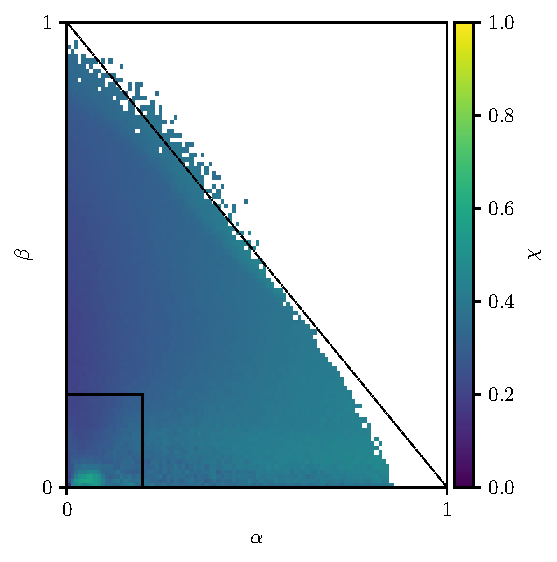
\includegraphics[width=0.5\textwidth]{figure/aphysical_chimera_100dpi.pdf}
  \caption[Chimera-like index landscape]{
    The chimera-like landscape of parameter space on $\pqty{\hra, \hrb} \in \pqty{0, 1.0} \times \pqty{0, 1.0}$.
    The aphysical region of the model is shown in white.
    The black rectangle in the bottom left corner indicates the region of parameter space shown in \cref{fig:zoom}.
    The dashed line has a slope of $-1$, to serve as a guide for \cref{sec:results_chimera}.
    The chimera-like index (defined in \cref{eq:chimera}) is normalized to 1, as usual.
  }
  \label{fig:aphysical_chimera}
\end{figure}
The boundary between physical and aphysical appears to be linear, with a negative slope.
This means that $\hra$ can range further when $\hrb$ is low,
and vice versa.
This makes sense, as increased $\hra$ and $\hrb$ influence the model in the same way (increasing the coupling and decreasing $\dot{\hrx}_{j}$).

Furthermore, the slope of the boundary is greater than $-1$, which means that $\hra$ has an greater influence on the physicality of the model.
This is also reasonable, but for slightly less self-evident reasons.
To explain why, we must look specifically at the coupling term from \cref{eq:hr_x}:
\[
  -\frac{\hra}{n'_{j}} \sum_{k = 1}^{N} G'_{j k} \Theta_{j}\pqty{\hrx_{k}}
  -
  \frac{\hrb}{n''_{j}} \sum_{k = 1}^{N} G''_{j k} \Theta_{j}\pqty{\hrx_{k}}.
\]
This coupling will, in fact, be positive, as $\Theta_{j}\pqty{\hrx_{k}} < 0$ if $\hrx_{j} < 2$, which is true almost all of the time.
This means that, as $\hra$ and $\hrb$ increase, so does the overall coupling strength.
So, there is some threshold $K$ for which the overall coupling is too strong if, for some $j$,
\begin{equation}
  \label{eq:coupling_inequality}
  \frac{\hra}{n'_{j}} \sum_{k = 1}^{N} G'_{j k} \abs{\Theta_{j}\pqty{\hrx_{k}}}
  +
  \frac{\hrb}{n''_{j}} \sum_{k = 1}^{N} G''_{j k} \abs{\Theta_{j}\pqty{\hrx_{k}}}
  >
  K_{j}.
\end{equation}
In order for $\hra$ to influence the coupling's proximity to $K$ more than $\hrb$ does, there must exist some $j$ such that
$\frac{1}{n'_{j}} \sum G'_{j k} \abs{\Theta_{j}\pqty{\hrx_{k}}}
>
\frac{1}{n''_{j}} \sum G''_{j k} \abs{\Theta_{j}\pqty{\hrx_{k}}}$.
Seeing as $\overline{g}'_{j} = \frac{1}{n'_{j}} \sum G'_{j k}$ and $\overline{g}''_{j} = \frac{1}{n''_{j}} \sum G''_{j k}$ are the average connection strength within and between cortices (shown in \cref{fig:average_strengths} A), these are simply a function of the topology of the graph.

It may look from \cref{fig:average_strengths} A like $\hrb$ should have more influence than $\hra$, as for most $j$, $\overline{g}''_{j} > \overline{g}'_{j}$.
However, for most of those cases, $\overline{g}'_{j_{0}} > \overline{g}''_{j_{0}} = 0$.
This means that, for those $j_{0}$, $\pdv{K_{j_{0}}}{\hra} = 0$.
So, those cases contribute to the value of the threshold, but do not influence the physicality's dependence on $\hra$ and $\hrb$.

If we remove the $j$ for which $0 \in \Bqty{\overline{g}'_{j}, \overline{g}''_{j}}$, we find that, on average, $\overline{g}'_{j} = 2.100$, slightly more than $\overline{g}''_{j} = 2.079$ (see \cref{fig:average_strengths} B).
This explains the slope of the boundary between the physical region and the aphysical region.

%%% Local Variables:
%%% mode: latex
%%% TeX-master: "../../ms"
%%% End:
